\documentclass[main.tex]{subfiles}
\begin{document}
	\chapter{結果}
	
	\section{アウトフローの確認}
	subhalo342447について図\ref{fig:outflowsubhalo342447}に示すようにアウトフローを確認した.一方でsubhalo388544はアウトフローが確認できず,subhalo421555は下向きの片方のみ確認できた (図\ref{fig:outflowsubhalo}).
	
	
	\begin{figure}[htbp]
		\centering
		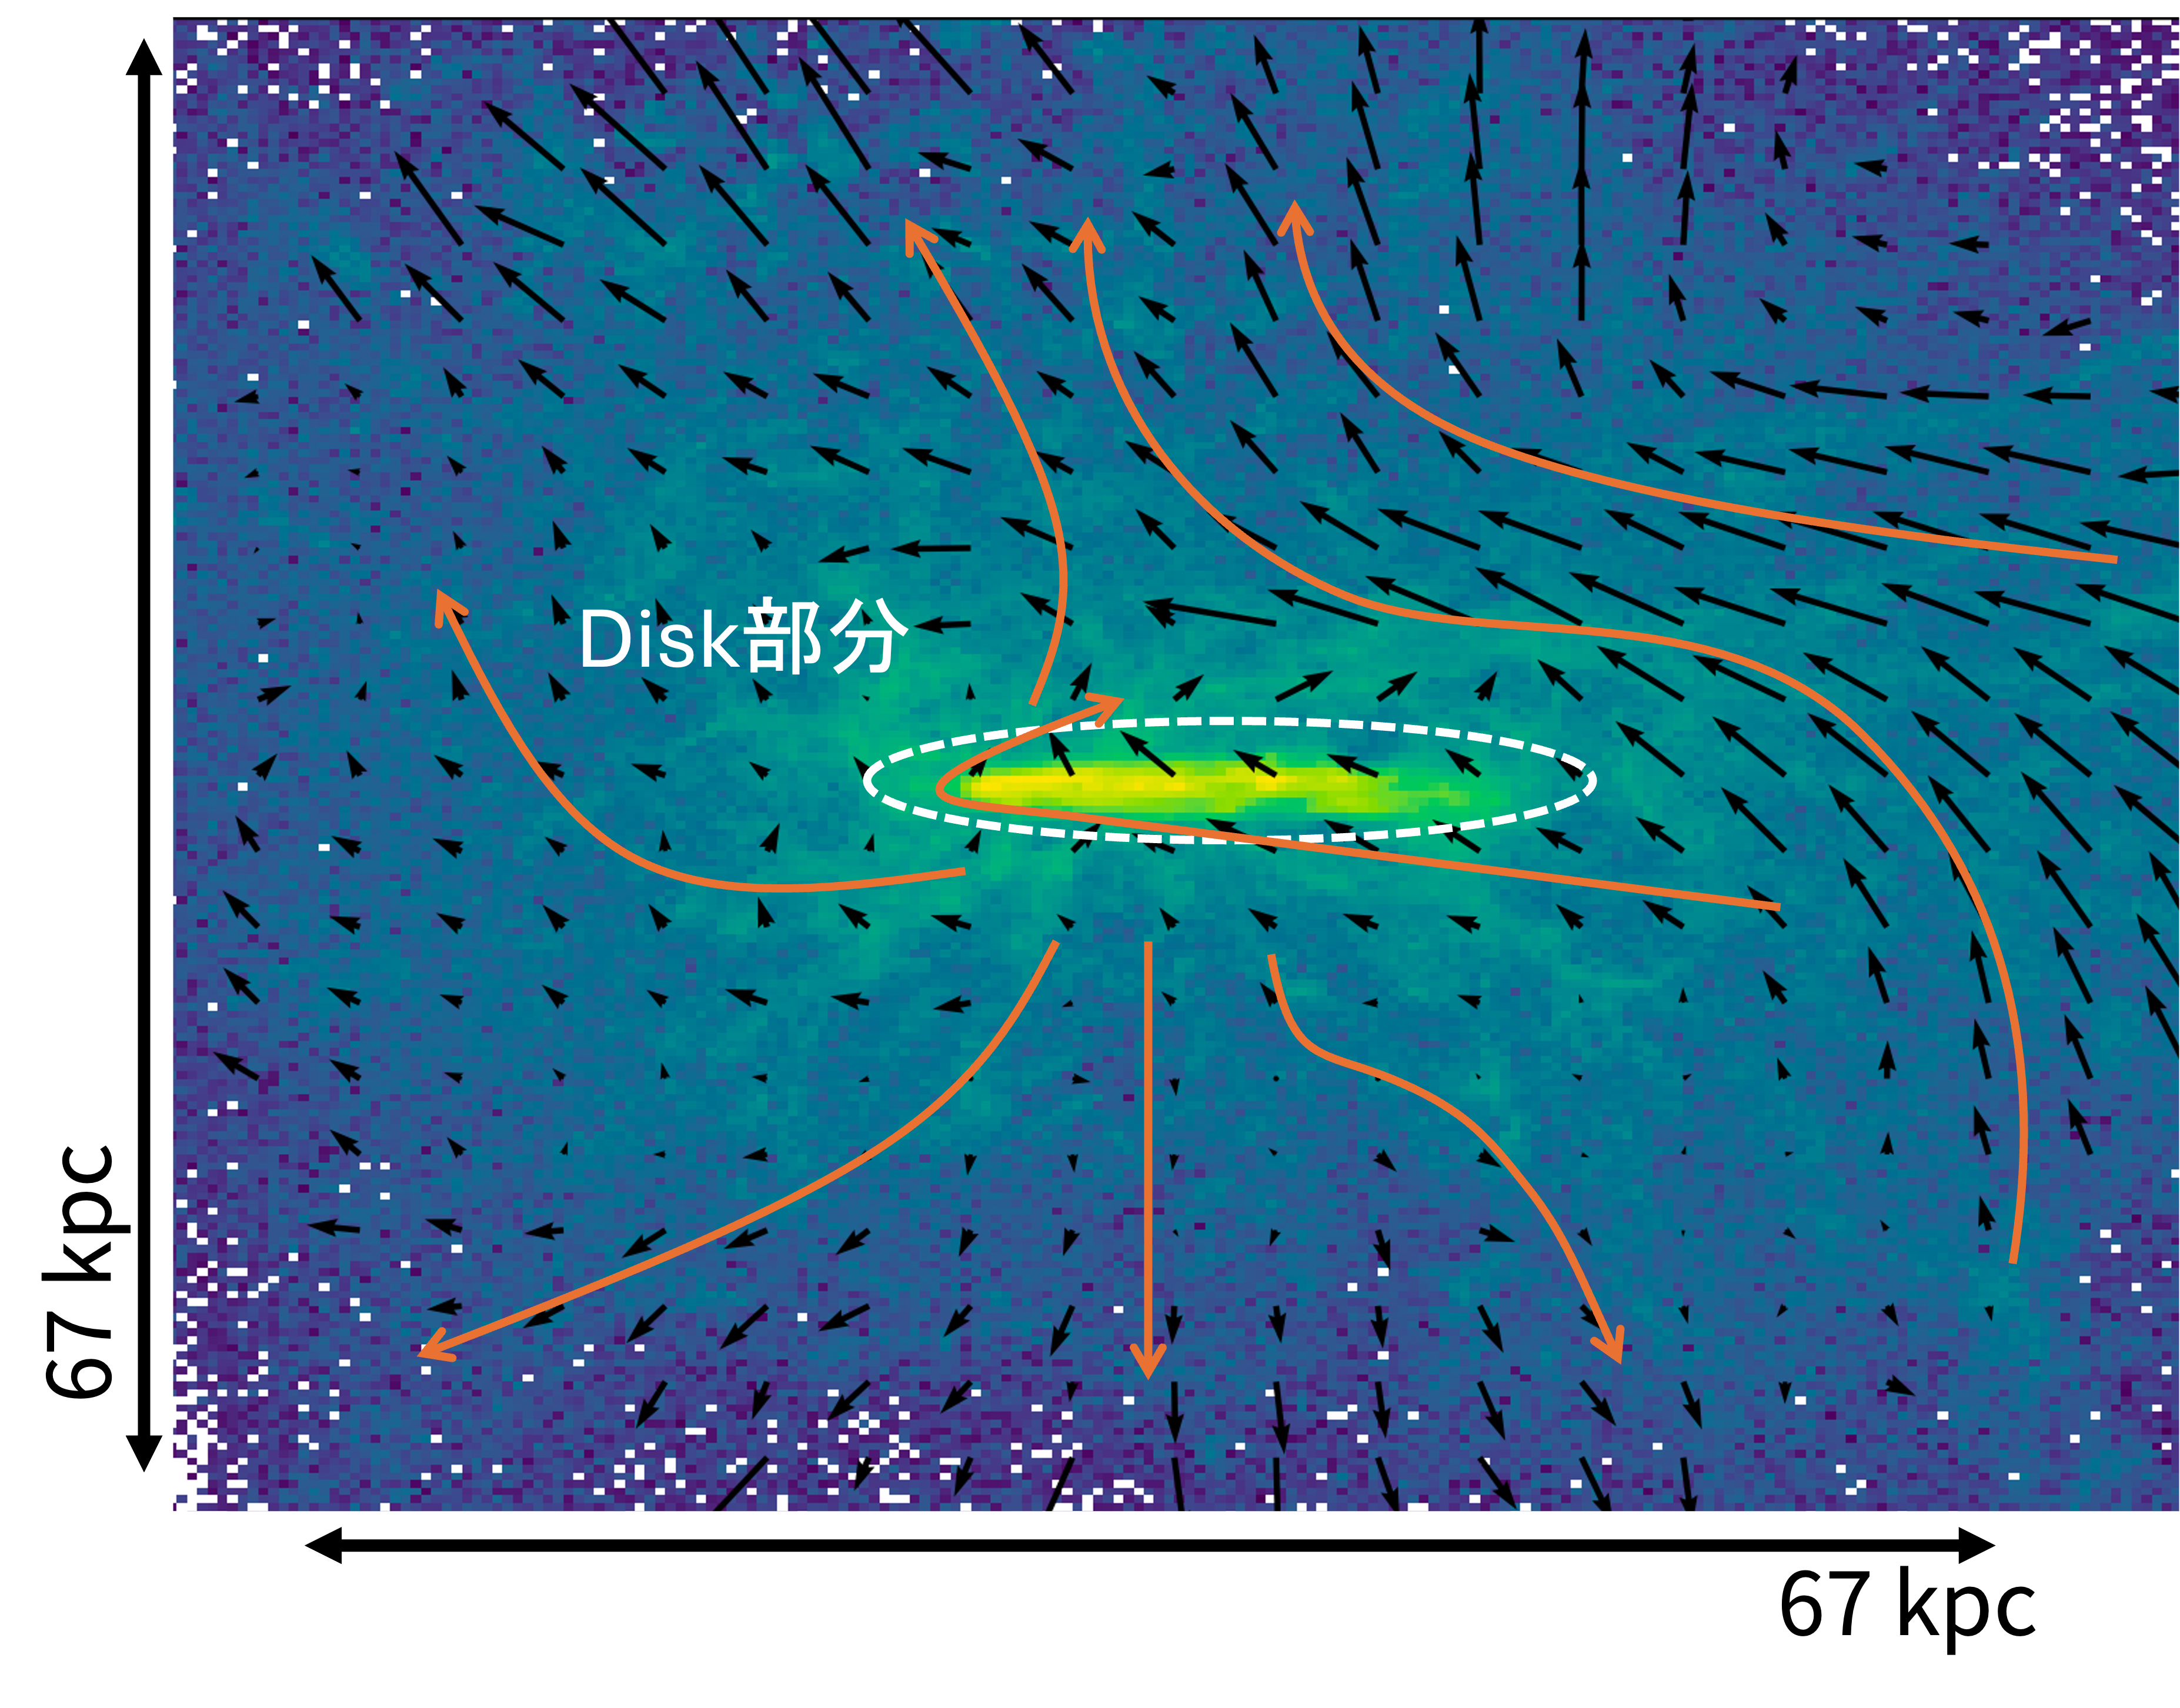
\includegraphics[width=0.6\linewidth]{pic/outflow_subhalo342447}
		\captionsetup{width=.8\linewidth}
		\caption{subhalo342447をedge-onで表示したもの.Massesを背景に表示して速度場を表示している.}
		\label{fig:outflowsubhalo342447}
	\end{figure}
	
	\begin{figure}[htbp]
		\centering
		\begin{minipage}[b]{0.45\linewidth}
			\centering
			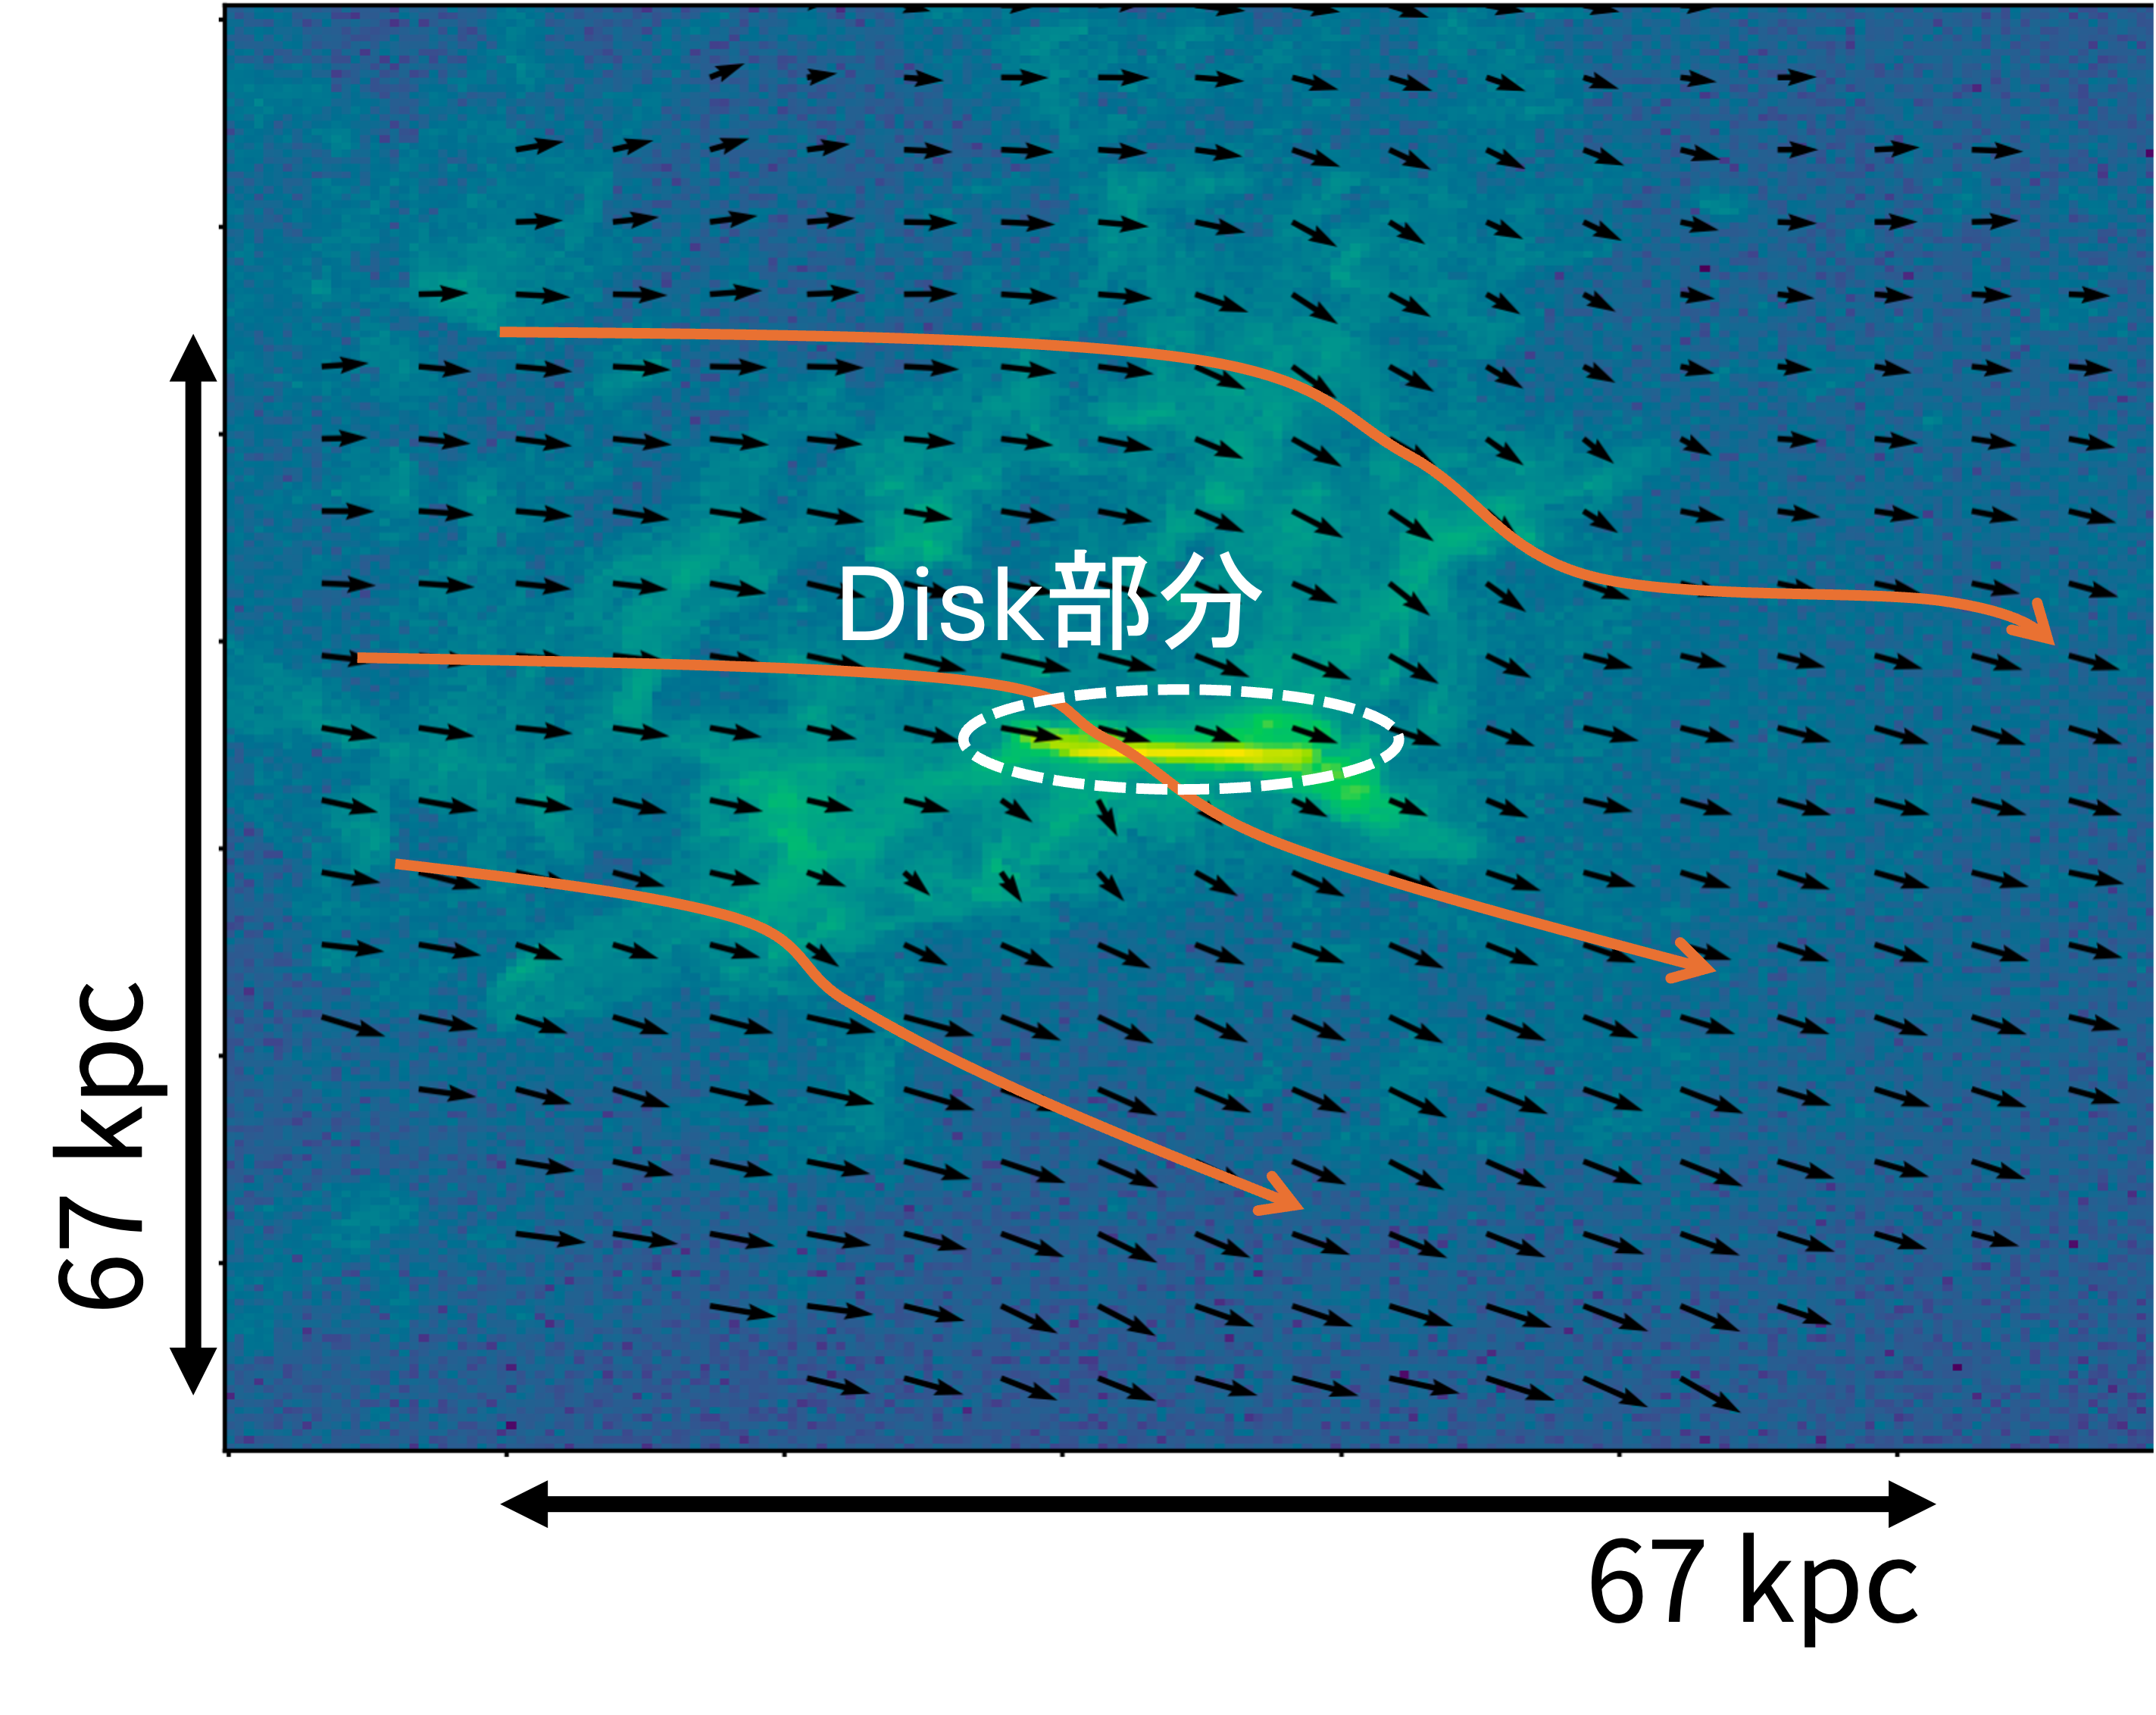
\includegraphics[width=\linewidth]{pic/outflow_subhalo388544}
			\subcaption{subhalo388544}
			\label{fig:outflowsubhalo388544}
		\end{minipage}
		\begin{minipage}[b]{0.45\linewidth}
			\centering
			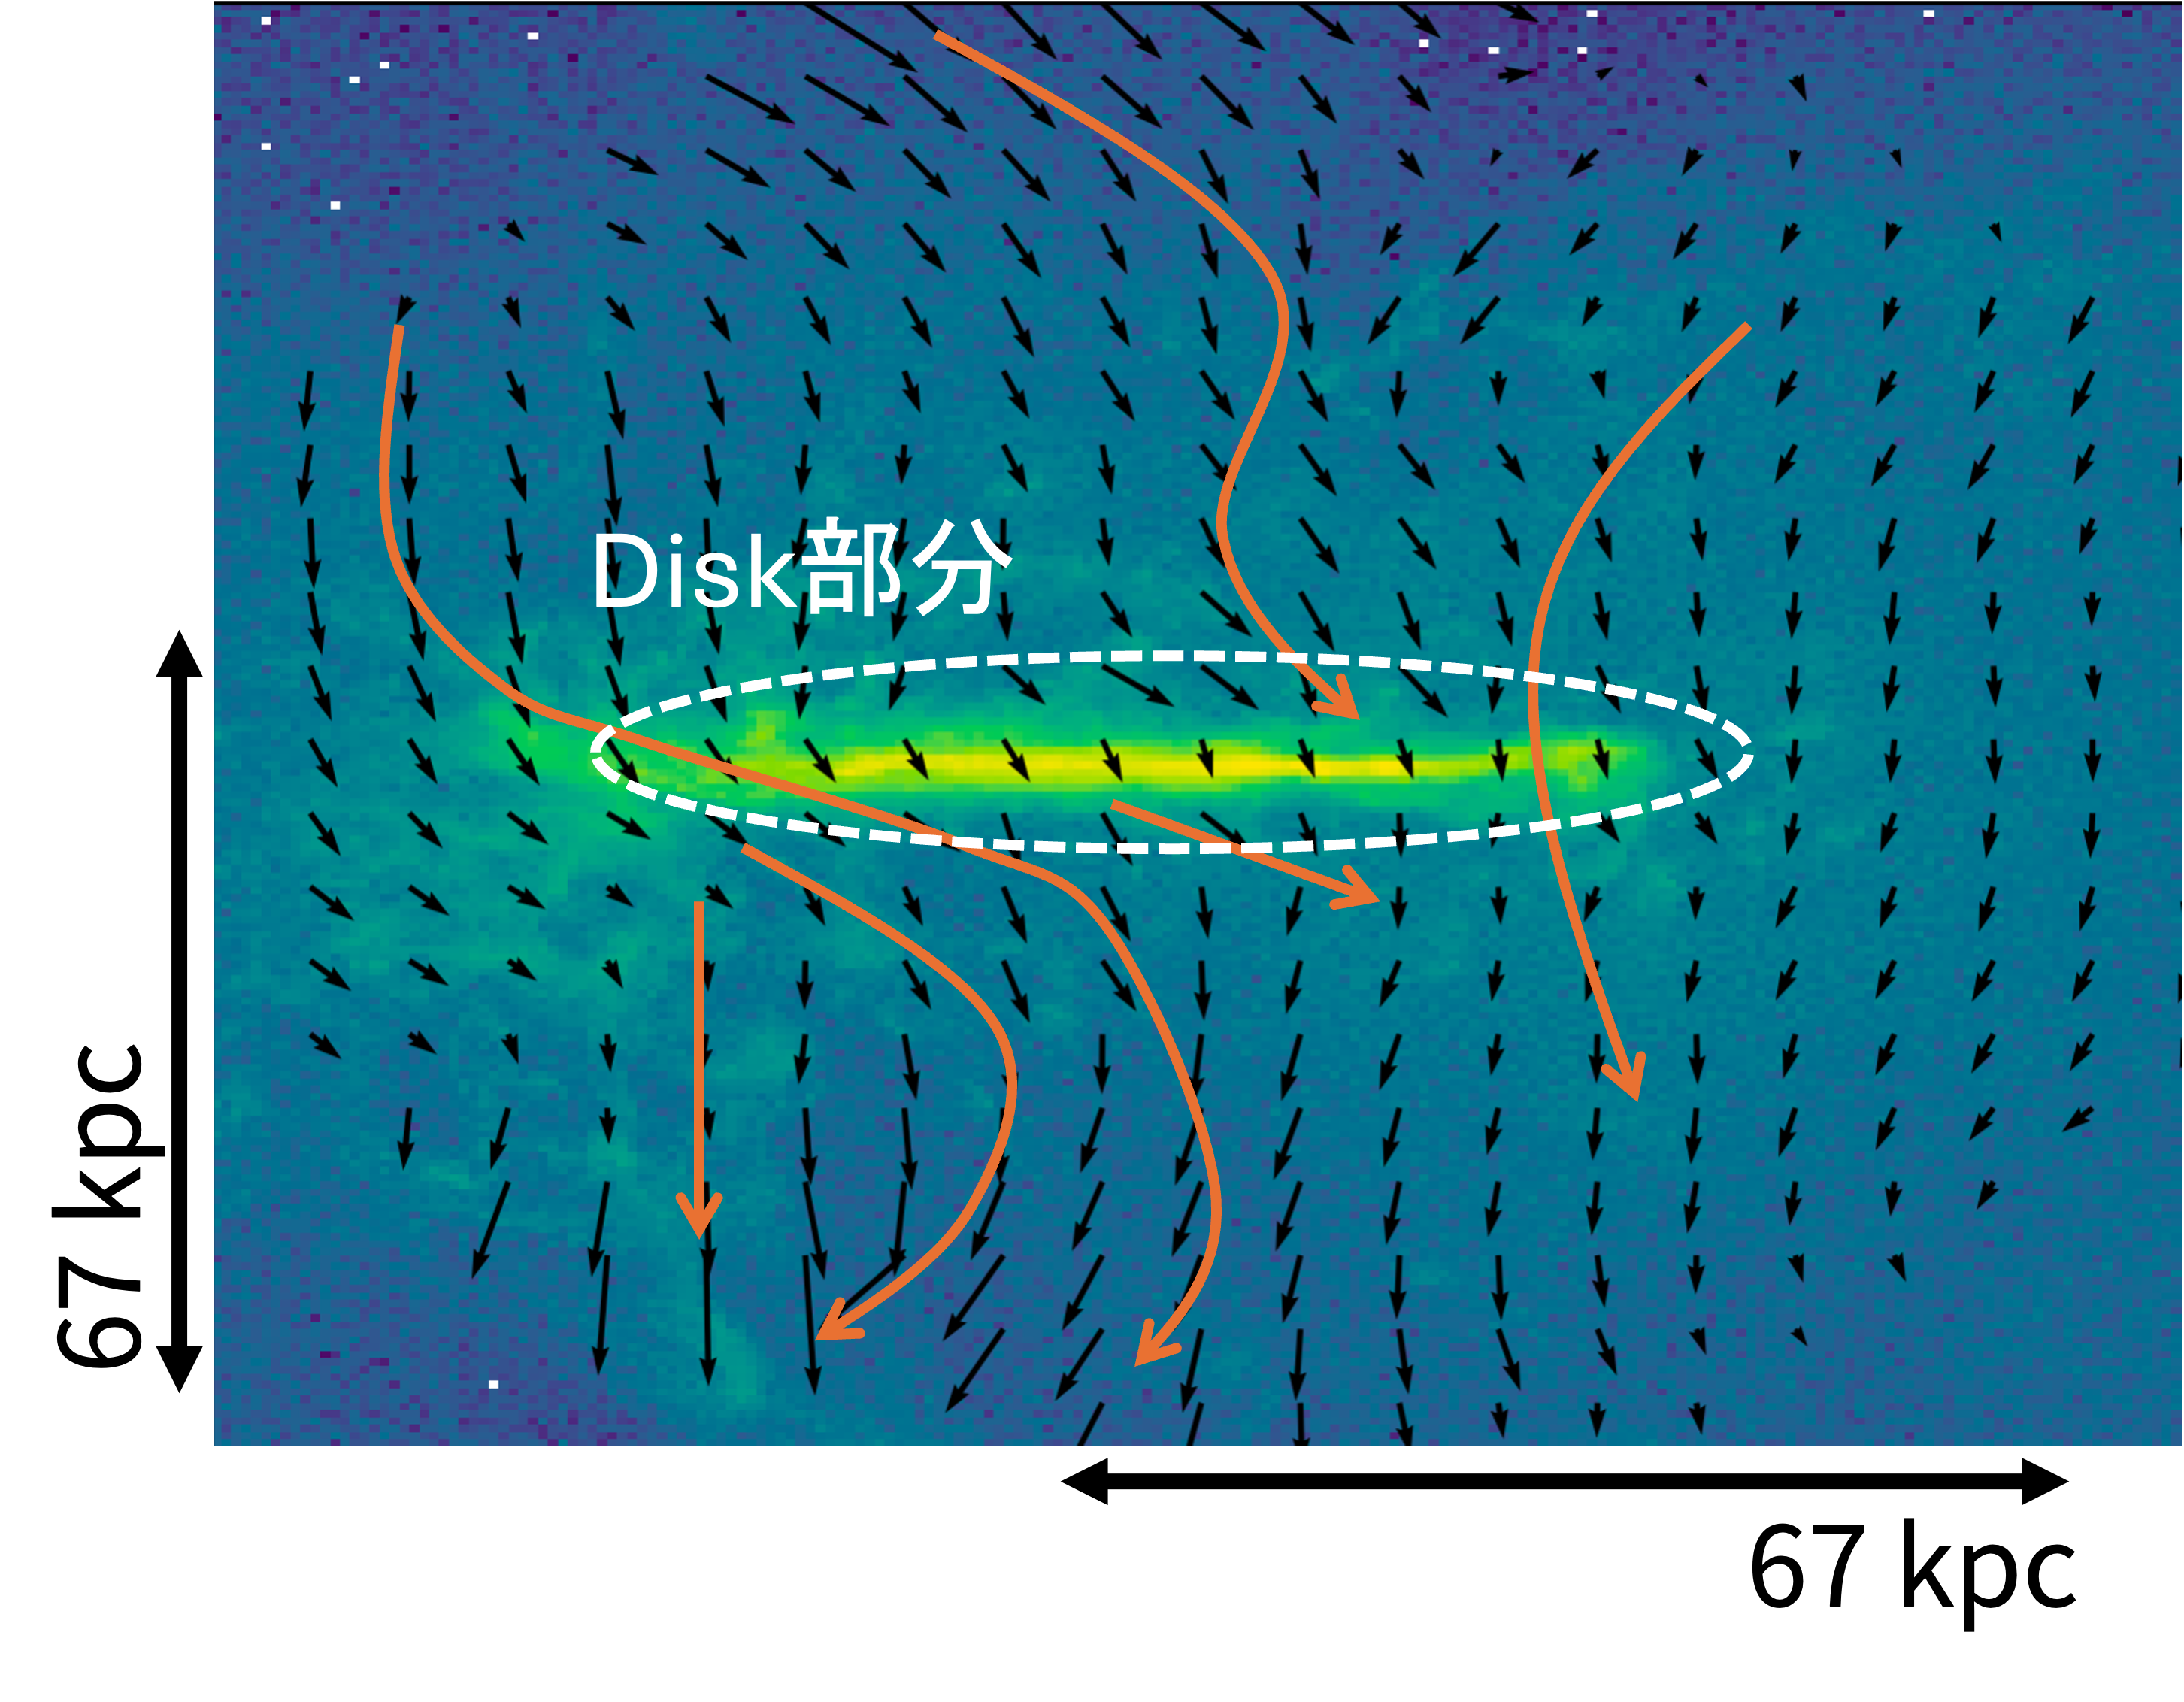
\includegraphics[width=\linewidth]{pic/outflow_subhalo421555}
			\subcaption{subhalo421555}
			\label{fig:outflowsubhalo421555}
		\end{minipage}
		\captionsetup{width=.9\linewidth}
		\caption{edge-onで表示.Massesを背景に表示して速度場を表示している.}
		\label{fig:outflowsubhalo}
	\end{figure}
	
	\section{動径方向の元素分布}
	
	subhao342447の動径方向の元素分布を図\ref{fig:abundanceprofile342447}に示す.R/R$_{200} < 0.1$においてsolar abundanceは,2倍程度であり,中心から外縁に向かうに連れて現象していった.
	
	\begin{figure}[htbp]
		\centering
		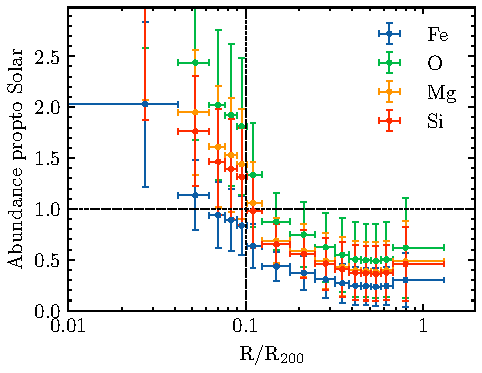
\includegraphics[width=0.6\linewidth]{pic/abundance_profile342447}
		\captionsetup{width=\linewidth}
		\caption{subhalo342447のFe, O, Mg, Siの太陽組成比を縦軸にし,横軸をsubhaloの中心(subhaloの移動質量中心で,subhalo内のすべての粒子/セルの質量加重相対座標の合計として計算される)からの距離をビリアル半径で規格化したものを片対数で表している.データは15個にグループまとめし,エラーバーは横軸がデータ幅(上限と下限),縦軸が標準偏差を表す.}
		\label{fig:abundanceprofile342447}
	\end{figure}
	
	一方でsubhalo388544とsubhalo421555においてR/R$_{200} < 0.1$では,太陽組成程度で中心から外縁部に向かって減少していることが分かった(図\ref{fig:2radicalprofile}).
	
	\begin{figure}[htbp]
		\centering
		\begin{minipage}[b]{0.45\linewidth}
			\centering
			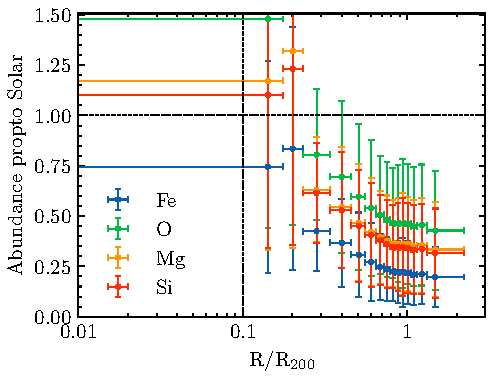
\includegraphics[width=\linewidth]{pic/abundance_profile388544}
			\subcaption{subhalo388544}
			\label{fig:abundanceprofile388544}
		\end{minipage}
		\begin{minipage}[b]{0.45\linewidth}
			\centering
			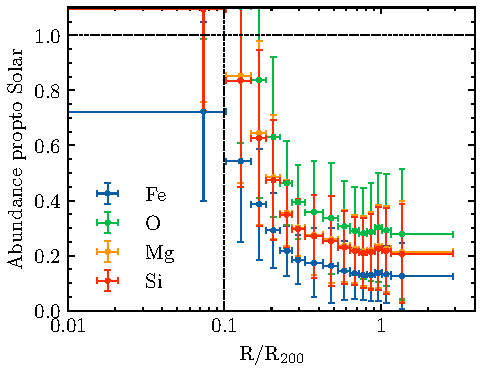
\includegraphics[width=\linewidth]{pic/abundance_profile421555}
			\subcaption{subhalo421555}
			\label{fig:abundanceprofile421555}
		\end{minipage}
		\caption{太陽組成比-対-ビリアル半径で規格化した半径.図\ref{fig:abundanceprofile342447}と同様}
		\label{fig:2radicalprofile}
	\end{figure}
	
	subhalo342447において,鉄の太陽組成比に対する酸素,ネオン,マグネシウムとケイ素の太陽組成比を計算したものを図\ref{fig:fe10}に示す.$\text{[O/Fe]} \sim 0.33$程度,$\text{[Ne/Fe]} \sim 0.53$程度,$\text{[Mg/Fe]} \sim 0.23$程度,$\text{[Si/Fe]} \sim 0.2$程度であった.図\ref{fig:fe10}では$0.1<\text{R/R}_{200} < 0.5$で他の部分と組成が異なる「へこみ」が観測された.
	
	\begin{figure}[htbp]
		\centering
		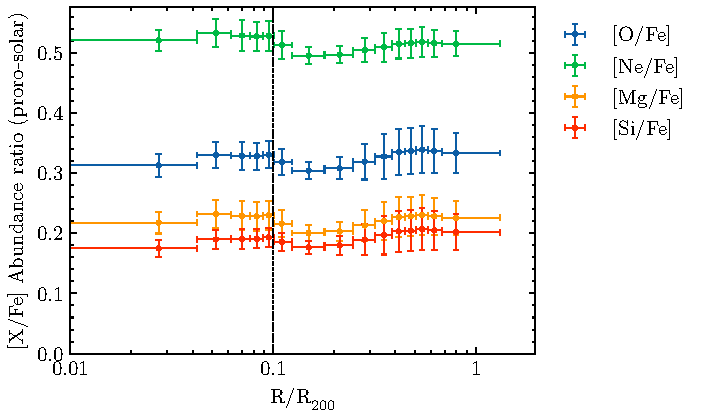
\includegraphics[width=0.8\linewidth]{pic/Fe10}
		\caption{subhalo342447の[X/Fe] (ただし X $=$O, Ne, Mg, Si)を縦軸にし,横軸をsubhaloの中心(subhaloの移動質量中心で,subhalo内のすべての粒子/セルの質量加重相対座標の合計として計算される)からの距離をビリアル半径で規格化したものを片対数で表している.データは15個にグループまとめし,エラーバーは横軸がデータ幅(上限と下限),縦軸が標準偏差を表す.}
		\label{fig:fe10}
	\end{figure}
	
	\section{温度分布}
	
	subhalo342447の温度分布を図\ref{fig:atemp}に示す.図\ref{fig:atemp}の右側で,R/R$_{200} < 0.1$においては\SI{e6}{K}以上の高温ガスが確認できた.左側は\num{1e+5}から\SI{4e+5}{K}の範囲の比較的低い温度が観測された.温度分布は左右で非対称であることが確認できる.
	
	また明らかに銀河の腕部分は\SI{e5}{K}以下と非常に低温なガスであることが確認できる.
	
	\begin{figure}[htbp]
		\centering
		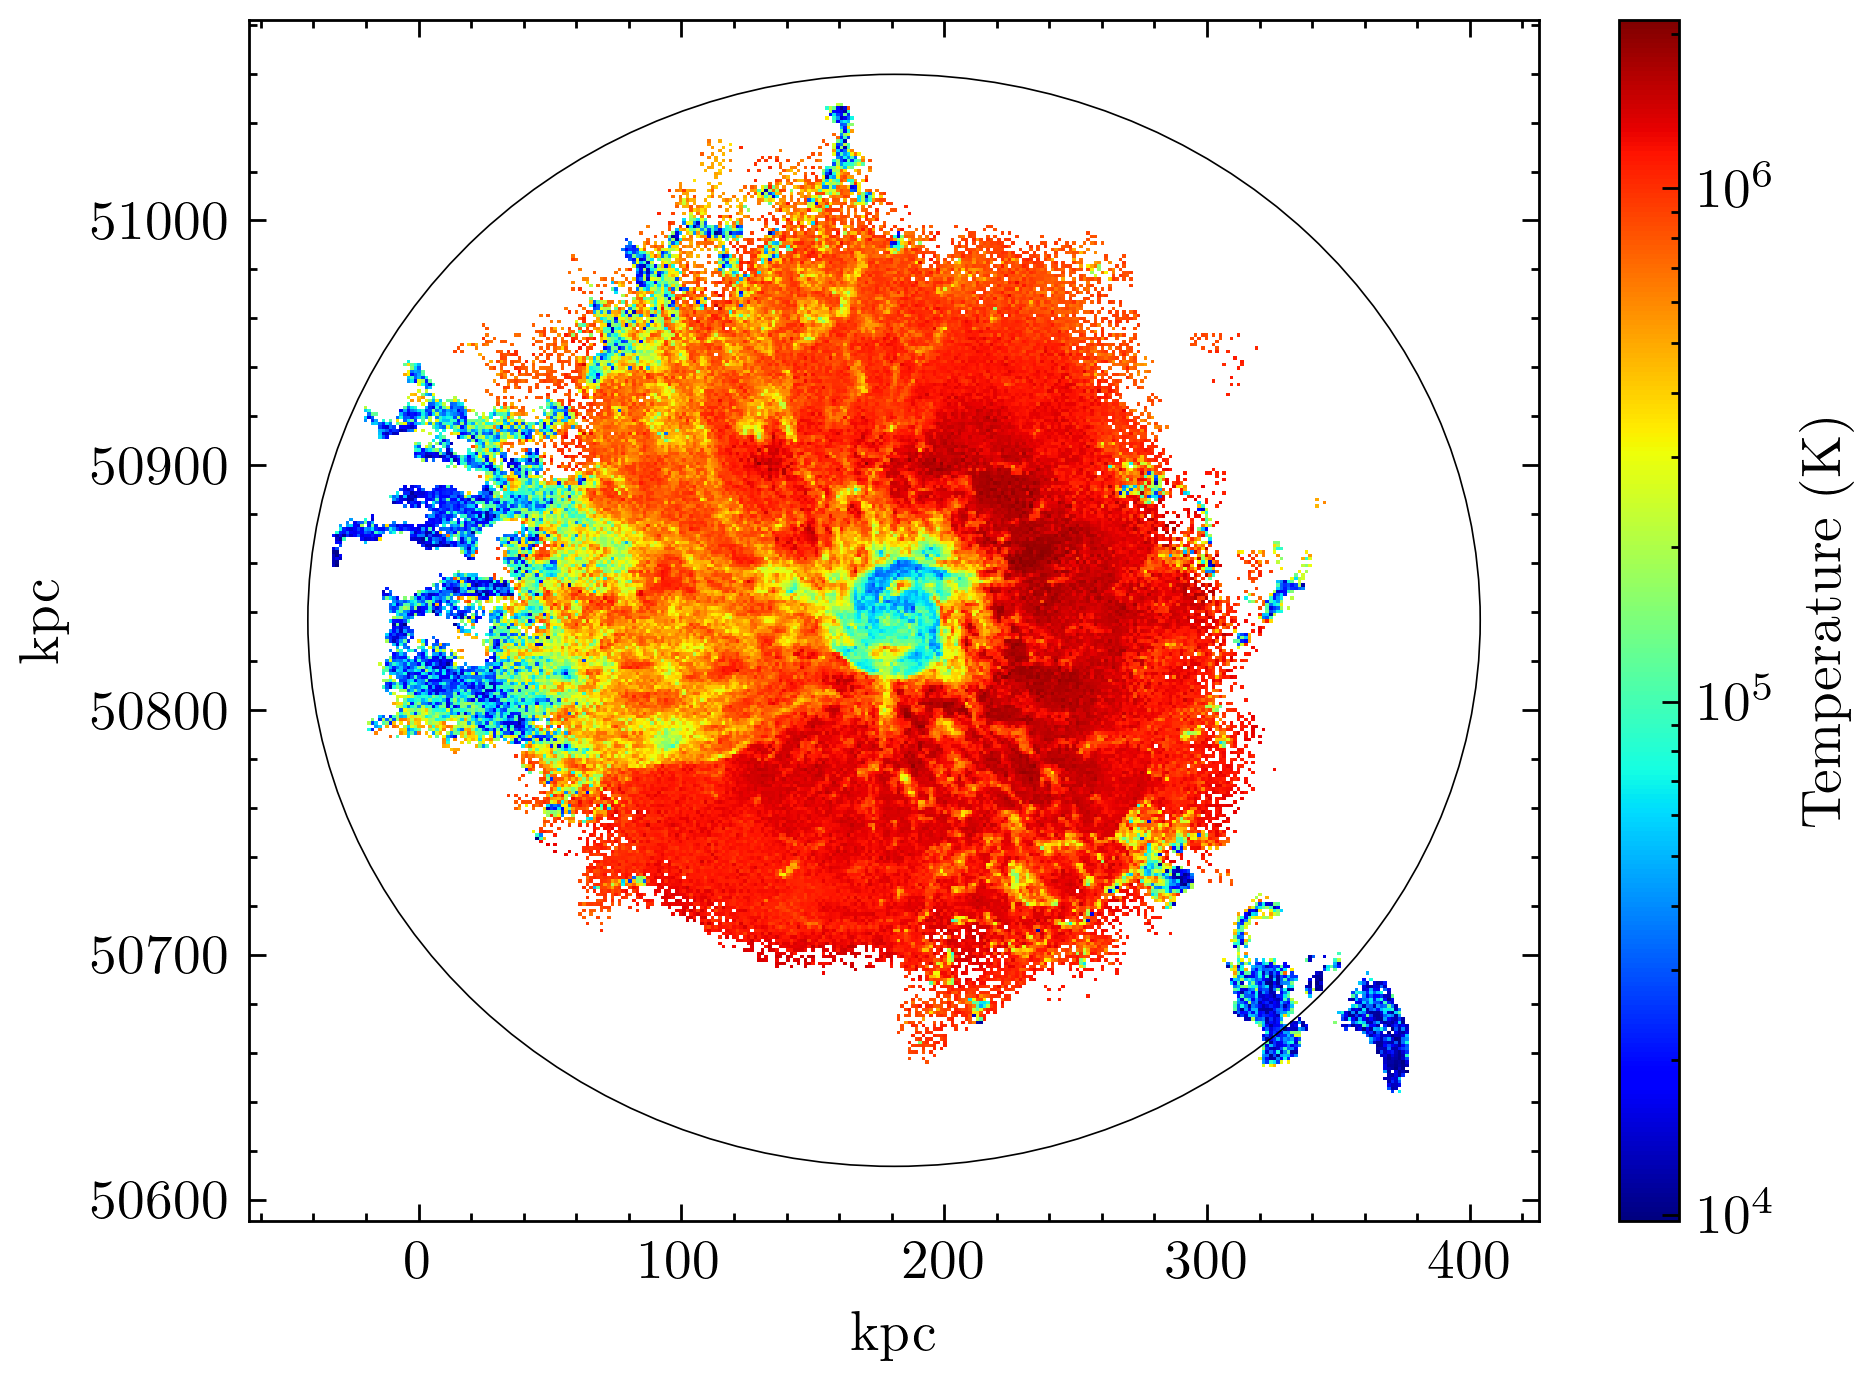
\includegraphics[width=0.8\linewidth]{pic/a_temp}
		\captionsetup{width=0.9\linewidth}
		\caption{face-on表示にしたsubhalo342447を各メッシュ内の平均温度を表している.円はビリアル半径を表す.計算にはガスのみを対象とした.}
		\label{fig:atemp}
	\end{figure}

\end{document}
